\documentclass{beamer}

\usepackage[british]{babel}
\usepackage{graphicx,hyperref,ru,url}

% Objective of the paper: what is the goal of this work? what problem is addressed? what was the current state of the art? who is the work aimed at?
% Proposal made in the paper: what is the new idea presented? what contributions does the paper claim to make? which one do you consider the most significant?
% Evidence given: how does the paper attempt to support its claims? through theorems/case studies/simulations/benchmarks? does the provided evidence indeed support the claims made?
% Shoulders of giants: what previous research does this work build on? what are the key underlying theoretical ideas? could this work have been done earlier?
% Impact: has this work been influential? what contribution do later papers mainly refer to? is the work still relevant or has it been superceded? is money being made from this idea?
% Discussion points (for presentation): give a number of questions, possibly including those emailed to you by your fellow students, which should arise in the discussion that follows.
% Discussion (for review): summarize the discussion during the meeting.


% The title of the presentation:
%  - first a short version which is visible at the bottom of each slide;
%  - second the full title shown on the title slide;
\title[Generation of undirected responses]{
  Generation of undirected responses}

% Optional: a subtitle to be dispalyed on the title slide
\subtitle{Learning models on Reddit data}

% The author(s) of the presentation:
%  - again first a short version to be displayed at the bottom;
%  - next the full list of authors, which may include contact information;
\author[Group 7]{
  Bauke Brenninkmeijer, Wietse Kuipers and Ties Robroek}
  % \\\medskip
  % {\small \url{ties.robroek@student.ru.nl}}}

% The institute:
%  - to start the name of the university as displayed on the top of each slide
%    this can be adjusted such that you can also create a Dutch version
%  - next the institute information as displayed on the title slide
\institute[Radboud University Nijmegen]{
  Institute for Computing and Information Sciences \\
  Radboud University Nijmegen}

% Add a date and possibly the name of the event to the slides
%  - again first a short version to be shown at the bottom of each slide
%  - second the full date and event name for the title slide
\date[14th of June, 2018]{
  14th of June, 2018}

\begin{document}

\begin{frame}
  \titlepage
\end{frame}

\begin{frame}
  \frametitle{Outline}

  \tableofcontents
\end{frame}

% Section titles are shown in at the top of the slides with the current section
% highlighted. Note that the number of sections determines the size of the top
% bar, and hence the university name and logo. If you do not add any sections
% they will not be visible.
\section{Introduction}

\begin{frame}
  \frametitle{Introduction}

  \begin{itemize}
    \item Can we learn a bot to write "proper" reddit comments?
    \item Various subreddits.
  \end{itemize}
\end{frame}

\section{Dataset}

\begin{frame}
  \frametitle{Dataset}

  \begin{itemize}
    \item the\_donald
    \item politics
    \item askreddit
  \end{itemize}
\end{frame}



\section{Model}

\begin{frame}
  \frametitle{Model}

  \begin{itemize}
    \item Markov Chain
    \item RNN
    \item GAN
  \end{itemize}
\end{frame}

\begin{frame} [fragile]
  \frametitle{Markov Chain}
  \begin{figure}[h]
  \center
  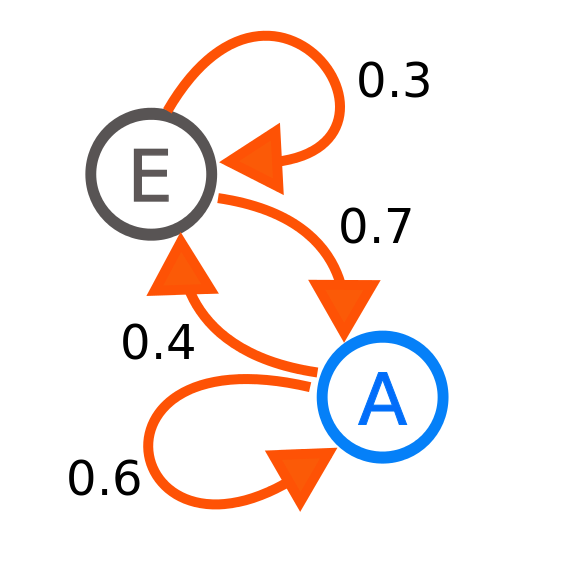
\includegraphics[width=0.4\textwidth]{markov}
  \end{figure}
\end{frame}

\begin{frame} [fragile]
  \frametitle{RNN}

  \begin{figure}[h]
  \center
  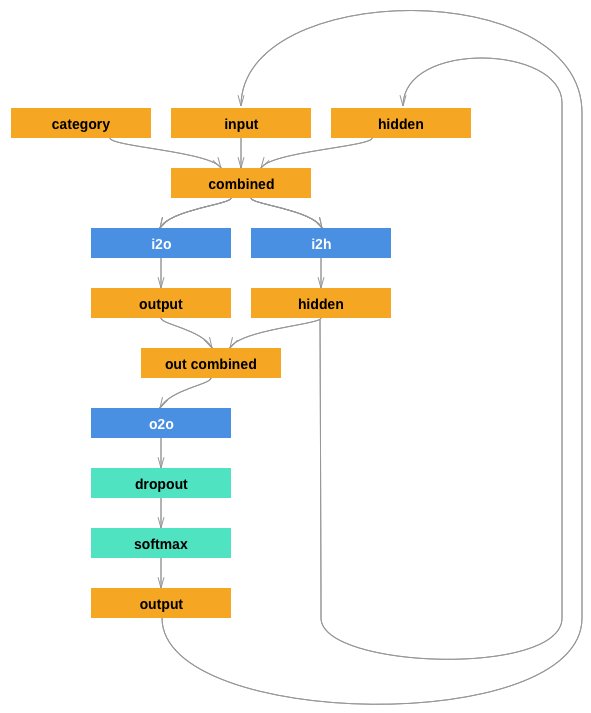
\includegraphics[width=0.5\textwidth]{rnn}
  \end{figure}
\end{frame}

\begin{frame} [fragile]
  \frametitle{GAN}

  \begin{figure}[h]
  \center
  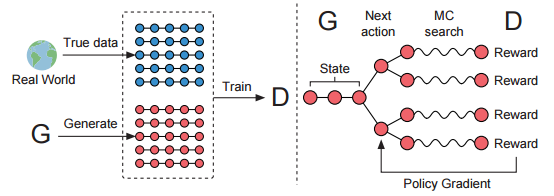
\includegraphics[width=\textwidth]{seqgan}
  \end{figure}
\end{frame}

\section{Training}

\begin{frame}
  \frametitle{Training}

  \begin{itemize}
    \item Models are extremely sensitive to "errors" and variation
    \item Termcount
    \item Dictionary filter
  \end{itemize}
\end{frame}

\section{Future}

\begin{frame}
  \frametitle{Future}

  \begin{itemize}
    \item Finalize cleaning of dataset
    \item Run GAN for a day
    \item Test results
  \end{itemize}
\end{frame}

\section{Conclusion}

\begin{frame}
  \frametitle{Conclusion}

  \begin{Conclusion}
    \textit{its like watching a movie coming out as a possible republican candidate who had a mad crush on her being responsible for the worthless rinos on the peoples of europe sounds familiar}
  \end{itemize}
  % {\tiny
  % \begin{verbatim}
  % Convolutional Deep Belief Networks on CIFAR-10, Alex Krizhevsky, 2010
  % \end{verbatim}
  % }
\end{frame}


\end{document}
